\documentclass[12pt, a4paper]{article}

% ─── Pacotes Fundamentais ────────────────────────────────────────────────────
\usepackage[utf8]{inputenc}
\usepackage[T1]{fontenc}
\usepackage[brazil]{babel}
\usepackage{geometry}
\usepackage{graphicx}
\usepackage{booktabs}
\usepackage{array}
\usepackage{longtable}
\usepackage{multirow}
\usepackage{hyperref}
\usepackage{xcolor}
\usepackage{listings}
\usepackage{amsmath}
\usepackage{amssymb}
\usepackage{enumitem}
\usepackage{float}
\usepackage{caption}
\usepackage{subcaption}
\usepackage{tikz}
\usetikzlibrary{positioning}
\usepackage{parskip}
\usepackage{fancyhdr}
\setlength{\headheight}{14pt}

% ─── Configurações de Página ─────────────────────────────────────────────────
\geometry{
  top=2.5cm,
  bottom=2.5cm,
  left=3.0cm,
  right=2.5cm
}
\setlength{\parskip}{0.55em}
\setlength{\parindent}{0pt}

% ─── Cores Institucionais ────────────────────────────────────────────────────
\definecolor{ufalblue}{RGB}{0, 60, 113}
\definecolor{codebg}{RGB}{247, 248, 250}
\definecolor{coderule}{RGB}{220, 224, 230}

% ─── Listings ────────────────────────────────────────────────────────────────
\lstset{
  backgroundcolor=\color{codebg},
  basicstyle=\small\ttfamily,
  breaklines=true,
  captionpos=b,
  commentstyle=\color{gray},
  frame=single,
  rulecolor=\color{coderule},
  keywordstyle=\color{ufalblue}\bfseries,
  stringstyle=\color{teal},
  showstringspaces=false,
  numbers=left,
  numberstyle=\tiny\color{gray},
  xleftmargin=1.5em,
  language=Python
}

% ─── Cabeçalho e Rodapé ──────────────────────────────────────────────────────
\pagestyle{fancy}
\fancyhf{}
\fancyhead[L]{\small\color{ufalblue}\textsc{ECOM031: Inteligência Artificial}}
\fancyhead[R]{\small\color{gray}UFAL / IC: Lista de Exercícios 2}
\fancyfoot[C]{\small\thepage}
\renewcommand{\headrulewidth}{0.4pt}

% ─── Configurações de Links ──────────────────────────────────────────────────
\hypersetup{
  colorlinks=true,
  linkcolor=ufalblue,
  urlcolor=ufalblue,
  citecolor=ufalblue
}

% ─── Identificação do Trabalho ───────────────────────────────────────────────
\title{
  {\large\textbf{UNIVERSIDADE FEDERAL DE ALAGOAS (UFAL)}}\\[0.2em]
  {\large\textbf{INSTITUTO DE COMPUTAÇÃO / ENGENHARIA DE COMPUTAÇÃO}}\\[1.5em]
  {\Large\bfseries\color{ufalblue} Lista de Exercícios 2: Inteligência Artificial}\\[0.4em]
  {\normalsize Componente Curricular: ECOM031 (Graduação / PPGI)}
}
\author{
  \textbf{Bruno Gomes de Barros Filho}, matrícula 21111360\\[0.3em]
  \textbf{Antonio Rodrigo Lima de Andrade Tenório}, matrícula 23210707
}
\date{
  Professor: Evandro de Barros Costa\\[0.3em]
  Maceió, AL, 2026.2
}

\begin{document}

\maketitle
\thispagestyle{empty}
\vspace{1em}
\hrule
\vspace{1.5em}

\tableofcontents
\newpage

% ══════════════════════════════════════════════════════════════════════════════
\section{Questão 1: Ontologias versus grafos de conhecimento}
\label{sec:q1}
% ══════════════════════════════════════════════════════════════════════════════

Ontologias e grafos de conhecimento são duas formas de representar informações e relacionamentos entre diferentes entidades. Apesar de utilizarem estruturas semelhantes, com nós, relações e propriedades, cada abordagem possui características próprias e atende a necessidades diferentes. Enquanto as ontologias dão maior atenção à definição formal dos conceitos e às regras que relacionam esses conceitos, os grafos de conhecimento priorizam a organização das informações e as conexões entre os dados.

Para entender melhor essas diferenças, é importante observar como cada abordagem representa o conhecimento, realiza inferências e lida com grandes volumes de informação.

\subsection{Comparativo: principais diferenças entre as abordagens}

A diferença entre ontologias e grafos de conhecimento vai além da maneira como os dados são organizados. Ela também está relacionada à interpretação das informações, às regras utilizadas e ao tipo de consulta que cada modelo permite realizar.

\subsubsection{Formalismo lógico e hipótese de mundo}

As ontologias utilizam como fundamento as Lógicas de Descrição (\textit{Description Logics}), que fornecem uma base matemática para definir conceitos, propriedades e restrições. Um exemplo de padrão baseado nessa abordagem é o OWL~2. Nele, os elementos do domínio são descritos por meio de axiomas, permitindo estabelecer relações e regras que podem ser verificadas automaticamente.

Uma característica importante é a Hipótese de Mundo Aberto (\textit{Open World Assumption}, OWA). Nessa abordagem, quando uma informação não está registrada, não significa necessariamente que ela seja falsa. O sistema considera que aquele dado pode simplesmente não ser conhecido ou ainda não ter sido informado.

Outro aspecto é a ausência da pressuposição de nomes únicos (\textit{Non-Unique Name Assumption}). Isso significa que duas entidades com identificadores diferentes podem representar o mesmo indivíduo. Por exemplo, dois registros de uma pessoa podem ser considerados equivalentes por meio de uma relação como \texttt{owl:sameAs}, desde que existam informações que justifiquem essa equivalência.

Já nos grafos de conhecimento, especialmente nos modelos de propriedades rotuladas (\textit{Labeled Property Graphs}, LPG), como os utilizados pelo Neo4j, o foco costuma estar na consulta e na navegação entre as informações armazenadas. Em aplicações que seguem a Hipótese de Mundo Fechado (\textit{Closed World Assumption}, CWA), considera-se que os dados não encontrados na base não estão disponíveis para aquela consulta.

É importante destacar que essa diferença depende da tecnologia utilizada. Grafos baseados em RDF, por exemplo, também podem seguir a semântica de mundo aberto. Portanto, não se pode afirmar que todo grafo de conhecimento utiliza obrigatoriamente a hipótese de mundo fechado.

\subsubsection{Mecanismos de inferência: dedução e navegação}

Outra diferença importante está na maneira como cada abordagem trabalha com as informações.

Nas ontologias, a inferência é baseada em deduções lógicas. Para isso, são utilizados programas chamados \textit{reasoners}, como HermiT, Pellet e FaCT++, que analisam os axiomas definidos no modelo. Esses mecanismos conseguem identificar relações que não foram cadastradas diretamente, verificar inconsistências e classificar automaticamente os indivíduos de acordo com as regras existentes.

Entre as principais tarefas realizadas estão:
\begin{itemize}[leftmargin=2em]
  \item \textbf{Verificação de consistência:} identifica se existem informações contraditórias na ontologia.
  \item \textbf{Classificação:} organiza automaticamente as classes de acordo com as relações de especialização e generalização.
  \item \textbf{Subsunção:} verifica se uma classe está contida em outra, ou seja, se todos os seus indivíduos também pertencem a uma classe mais abrangente.
  \item \textbf{Instanciação:} identifica a quais classes um indivíduo pertence, inclusive quando essa relação pode ser deduzida a partir dos axiomas.
\end{itemize}

Nos grafos de conhecimento, o trabalho geralmente está mais relacionado à consulta e à análise das conexões entre os dados. Em ferramentas como o Neo4j, é possível utilizar a linguagem Cypher para percorrer relacionamentos, encontrar caminhos entre entidades e identificar informações conectadas.

Além disso, existem técnicas que permitem descobrir relações que ainda não foram registradas explicitamente. Entre elas estão os \textit{embeddings} de grafos, como TransE e RotatE, e as Redes Neurais em Grafos (\textit{Graph Neural Networks}, GNNs). Esses métodos podem ser utilizados para prever conexões que provavelmente existem entre duas entidades, tarefa conhecida como \textit{link prediction}.

Assim, enquanto as ontologias se destacam pela aplicação de regras lógicas para deduzir informações, os grafos oferecem recursos para explorar relacionamentos e identificar padrões presentes na rede.

\subsubsection{Escalabilidade e custo de processamento}

O nível de formalização das ontologias também influencia o custo de processamento. Quanto mais complexas forem as regras e relações definidas, maior pode ser o esforço necessário para realizar as inferências.

Em fragmentos expressivos do OWL~2~DL, alguns problemas de raciocínio apresentam complexidade computacional elevada, podendo chegar a níveis como NEXPTIME e 2EXPTIME. Por isso, executar inferências complexas sobre bases com centenas de milhões de instâncias pode exigir muitos recursos e não ser adequado para consultas em tempo real.

Nos grafos de propriedades, a estrutura de relacionamentos permite percorrer conexões diretamente, sem precisar analisar toda a base a cada consulta. No Neo4j, por exemplo, o conceito de \textit{index-free adjacency} permite que os nós mantenham referências diretas aos seus relacionamentos, facilitando a navegação entre entidades conectadas.

Isso pode tornar consultas locais bastante eficientes, especialmente quando o objetivo é encontrar caminhos ou relacionamentos próximos. Entretanto, o desempenho também depende da quantidade de conexões percorridas, da estrutura do grafo e da complexidade da consulta.

Na prática, a escolha entre as abordagens depende do objetivo da aplicação: quando a prioridade é validar regras e realizar deduções formais, as ontologias oferecem recursos adequados. Quando o objetivo é explorar grandes redes de relacionamentos e consultar conexões entre entidades, os grafos de conhecimento podem ser mais convenientes.

\begin{table}[H]
  \centering
  \caption{Síntese comparativa entre sistemas baseados em ontologias e grafos de conhecimento}
  \label{tab:comparativo_q1}
  \renewcommand{\arraystretch}{1.25}
  \small
  \resizebox{\textwidth}{!}{%
  \begin{tabular}{@{}p{3.4cm}p{5.6cm}p{5.8cm}@{}}
    \toprule
    \textbf{Dimensão de análise} & \textbf{Sistemas baseados em ontologias} & \textbf{Sistemas baseados em grafos de conhecimento} \\
    \midrule
    Núcleo teórico & Lógicas de Descrição (DL) e semântica formal & Teoria dos grafos e propriedades rotuladas (LPG) \\
    Ferramentas comuns & OWL~2, Protégé, HermiT e Pellet & Neo4j, Cypher, Amazon Neptune e RDF/SPARQL \\
    Hipótese de mundo & Geralmente Mundo Aberto (OWA) & Depende da tecnologia; LPGs frequentemente utilizam Mundo Fechado (CWA) \\
    Tipo de inferência & Dedução lógica baseada em axiomas & Navegação, análise de caminhos e métodos estatísticos \\
    Principal desafio & Custo computacional de inferências complexas & Manutenção da consistência e qualidade dos relacionamentos \\
    \bottomrule
  \end{tabular}%
  }
\end{table}

\subsection{Exemplo prático: catálogo e recomendação de filmes}

Para visualizar melhor como essas abordagens funcionam, podemos considerar um sistema de recomendação de filmes. A ideia é utilizar informações sobre diretores, atores, gêneros e produções para sugerir títulos de acordo com os interesses de cada usuário.

\subsubsection{Abordagem por ontologia: conceitos e regras}

Na construção da ontologia, inicialmente são definidas as classes que representam os elementos do domínio. Por exemplo:
\begin{itemize}[leftmargin=2em]
  \item \texttt{Pessoa}, representando pessoas envolvidas na produção cinematográfica;
  \item \texttt{Diretor} e \texttt{Ator}, como subclasses de \texttt{Pessoa}, declaradas disjuntas entre si;
  \item \texttt{Filme}, representando as produções cinematográficas;
  \item \texttt{dirigiu}, uma propriedade que relaciona um indivíduo da classe \texttt{Diretor} a um indivíduo da classe \texttt{Filme}.
\end{itemize}

Também podem ser definidas restrições para garantir que determinadas relações sejam utilizadas corretamente. Por exemplo, uma pessoa não pode ser classificada simultaneamente como \texttt{Diretor} e \texttt{Ator} caso o modelo tenha estabelecido essas classes como disjuntas.

A partir dessas definições, o \textit{reasoner} consegue deduzir novas informações. Se a base receber o fato de que \texttt{Christopher Nolan dirigiu Oppenheimer} e a propriedade \texttt{dirigiu} tiver domínio definido como \texttt{Diretor} e alcance definido como \texttt{Filme}, o sistema poderá inferir que Christopher Nolan pertence à classe \texttt{Diretor} e que Oppenheimer pertence à classe \texttt{Filme}.

Como \texttt{Diretor} é uma subclasse de \texttt{Pessoa}, também será possível concluir que Nolan pertence à classe \texttt{Pessoa}, sem que essa informação precise ser cadastrada diretamente.

Por outro lado, se a base registrar que \texttt{Inception} é o responsável por dirigir \texttt{Tenet}, o sistema poderá identificar uma inconsistência caso \texttt{Inception} esteja classificado como \texttt{Filme} e a propriedade exija que seu domínio seja \texttt{Diretor}. Nesse caso, o modelo identifica a incompatibilidade lógica, embora a detecção não signifique necessariamente que o registro será automaticamente rejeitado pelo sistema de armazenamento.

Dessa forma, a ontologia permite estabelecer regras sobre o domínio e verificar se as informações cadastradas estão de acordo com elas.

\subsubsection{Abordagem por grafo de conhecimento: conexões e consultas}

No grafo de conhecimento, a representação é feita por meio de entidades concretas e dos relacionamentos existentes entre elas. Por exemplo, podemos cadastrar \texttt{Steven Spielberg} (pessoa), \texttt{Jurassic Park} (filme) e \texttt{Ficção Científica} (gênero), conectados por arestas como \texttt{(:Pessoa)-[:DIRIGIU]->(:Filme)} e\\
\texttt{(:Filme)-[:GENERO]->(:Tema)}.

Com essa estrutura, o sistema consegue percorrer os relacionamentos e encontrar filmes que compartilham características com outros títulos. Quando um usuário demonstra interesse em \texttt{Jurassic Park}, uma consulta Cypher pode localizar outros filmes dirigidos pela mesma pessoa ou que possuam gêneros e características em comum. Nesse caso, o sistema pode encontrar títulos como \texttt{Tubarão} e \texttt{E.T.}, também dirigidos por Steven Spielberg. A recomendação acontece a partir das conexões existentes no grafo, sem a necessidade de utilizar um mecanismo de dedução lógica como o empregado nas ontologias.

\subsection{Mapeamento: da ontologia para o grafo de propriedades}

Na prática, também é possível utilizar as duas abordagens em conjunto. Uma possibilidade é desenvolver inicialmente o modelo conceitual no Protégé, utilizando OWL, e depois transportar sua estrutura para um banco de grafos, como o Neo4j.

Essa conversão exige alguns cuidados, pois nem todas as características de uma ontologia possuem uma representação direta em um grafo de propriedades. De maneira geral, o processo pode ser dividido em quatro etapas:

\begin{enumerate}[leftmargin=2em, label=\textbf{\arabic*.}]
  \item \textbf{Classes se tornam rótulos de nós (\textit{labels}).}
  Cada classe definida na ontologia pode ser representada por um rótulo no grafo. Por exemplo, as classes \texttt{Diretor} e \texttt{Pessoa} podem ser utilizadas como \textit{labels} de um mesmo nó. As hierarquias definidas por \texttt{subClassOf} também podem ser representadas dessa maneira, desde que a aplicação mantenha corretamente as relações entre as classes.

  \item \textbf{Propriedades de objeto se tornam relacionamentos.}
  As propriedades que representam relações entre entidades são convertidas em arestas direcionadas. Por exemplo, a propriedade \texttt{dirigiu} pode ser representada no grafo como \texttt{[:DIRIGIU]}.

  \item \textbf{Propriedades de dados se tornam atributos dos nós.}
  Informações como ano de lançamento, orçamento e título não precisam ser nós separados: podem ser armazenadas diretamente como atributos da entidade correspondente (\texttt{titulo}, \texttt{anoLancamento}, \texttt{orcamento}).

  \item \textbf{Axiomas e restrições precisam ser adaptados.}
  Bancos de grafos de propriedades não oferecem, nativamente, o mesmo mecanismo de raciocínio lógico das ontologias OWL. Algumas restrições podem ser representadas por \textit{constraints}, como regras de unicidade, enquanto outras precisam ser verificadas pela aplicação antes que os dados sejam armazenados. Regras de disjunção entre classes e determinadas restrições de cardinalidade precisam de validações adicionais para preservar a semântica do modelo original.
\end{enumerate}

A Figura~\ref{fig:mapeamento_ontologia_kg} ilustra esse mapeamento.

\begin{figure}[H]
  \centering
  \resizebox{\textwidth}{!}{%
  \begin{tikzpicture}[
      node distance=1.8cm,
      tboxnode/.style={draw, rectangle, rounded corners=3pt, fill=ufalblue!12,
                       minimum width=3.4cm, minimum height=0.9cm, font=\small\sffamily, align=center},
      aboxnode/.style={draw, rectangle, rounded corners=3pt, fill=green!15,
                       minimum width=3.6cm, minimum height=0.9cm, font=\small\sffamily, align=center},
      seta/.style={-stealth, thick, draw=ufalblue},
      meta/.style={font=\scriptsize\itshape, text=gray}
    ]
    \node[tboxnode] (c-dir) {\textbf{Classe OWL:}\\\texttt{Diretor}};
    \node[tboxnode, right=2.8cm of c-dir] (c-filme) {\textbf{Classe OWL:}\\\texttt{Filme}};
    \draw[seta] (c-dir) -- node[above, font=\scriptsize] {\texttt{ObjectProperty: dirigiu}} (c-filme);
    \node[draw, rectangle, fill=gray!15, below=1.4cm of c-filme, font=\small\ttfamily] (lit) {xsd:integer};
    \draw[seta] (c-filme) -- node[right, meta, align=left] {\texttt{DataProperty:}\\\texttt{anoLancamento}} (lit);
    \node[above=0.5cm of c-dir, font=\small\bfseries\color{ufalblue}] {Esquema terminológico (Ontologia OWL)};
    \draw[-stealth, very thick, gray, dashed]
          (3.8cm, -0.9cm) -- node[above, font=\footnotesize\bfseries] {Mapeamento} (5.6cm, -0.9cm);
    \node[aboxnode, right=5.8cm of c-dir] (n-dir) {\textbf{Nó LPG:}\\\texttt{(:Pessoa:Diretor)}\\{\scriptsize \{nome: "Steven Spielberg"\}}};
    \node[aboxnode, right=2.8cm of n-dir] (n-filme) {\textbf{Nó LPG:}\\\texttt{(:Filme)}\\{\scriptsize \{titulo: "Jurassic Park",}\\{\scriptsize anoLancamento: 1993\}}};
    \draw[seta, green!50!black] (n-dir) -- node[above, font=\scriptsize\bfseries] {\texttt{[:DIRIGIU]}} (n-filme);
    \node[above=0.5cm of n-dir, font=\small\bfseries\color{green!50!black}] {Estrutura instanciada (grafo de propriedades)};
  \end{tikzpicture}%
  }
  \caption{Mapeamento do modelo ontológico para grafo de propriedades rotuladas.}
  \label{fig:mapeamento_ontologia_kg}
\end{figure}

Como podemos observar, a ontologia fornece a estrutura conceitual e as regras que definem o domínio, enquanto o grafo representa as entidades e suas conexões de maneira adequada para consultas e exploração dos relacionamentos. As duas abordagens não precisam ser utilizadas de forma isolada: em determinadas aplicações, a combinação permite aproveitar a organização formal e a capacidade de inferência das ontologias, juntamente com a facilidade de navegação e consulta dos grafos de conhecimento.

\newpage

% ══════════════════════════════════════════════════════════════════════════════
\section{Questão 2: Classificador dos K-Vizinhos Mais Próximos (KNN)}
\label{sec:q2}
% ══════════════════════════════════════════════════════════════════════════════

\subsection{Base de dados e configuração do experimento}

O algoritmo dos $K$-Vizinhos Mais Próximos (\textit{K-Nearest Neighbors}, KNN) foi aplicado à mesma base de 30 instâncias de risco de crédito utilizada na Lista de Exercícios 1. A base tem como ponto de partida um exemplo apresentado no livro de Luger e foi ampliada na Questão~1 daquela lista, passando a contar com seis atributos categóricos e 30 exemplos, identificados de E1 a E30.

Os atributos utilizados para fazer as previsões são História de Crédito, Dívida, Garantia, Renda, Emprego e Imóvel. A variável que o modelo deve classificar é o risco de crédito, dividido em três categorias: Alto, Moderado e Baixo.

Como o KNN trabalha com medidas de distância numéricas, foi necessário transformar os atributos categóricos antes de aplicar o algoritmo. Para isso, utilizamos \textit{one-hot encoding} (\texttt{get\_dummies}), seguindo a mesma estratégia adotada no CART da Lista~1. Com essa transformação, cada categoria passou a ser representada por uma coluna binária, resultando em um conjunto de 14 dimensões com valores 0 ou 1.

Nesse formato, a distância euclidiana permite comparar os exemplos contando, de forma indireta, as diferenças entre suas categorias. Como todas as variáveis passaram a ter a mesma escala binária, não foi necessário aplicar normalização min-max.

Código e experimentos: \texttt{src/q02\_knn/q02\_knn.ipynb}.

\subsection{As 30 instâncias utilizadas no experimento}

A Tabela~\ref{tab:30_instancias} apresenta a base completa utilizada na Lista~1, que também serviu de entrada para este experimento.

\begin{table}[H]
  \centering
  \caption{As 30 instâncias de risco de crédito da Lista 1}
  \label{tab:30_instancias}
  \renewcommand{\arraystretch}{1.12}
  \scriptsize
  \begin{tabular}{cccccccc}
    \toprule
    \textbf{Ex.} & \textbf{História} & \textbf{Dívida} & \textbf{Garantia} & \textbf{Renda} & \textbf{Emprego} & \textbf{Imóvel} & \textbf{Risco} \\
    \midrule
E1  & Ruim          & Alta  & Nenhuma   & 0--15  & Instável & Alugado & Alto \\
E2  & Desconhecida  & Alta  & Nenhuma   & 15--35 & Instável & Alugado & Alto \\
E3  & Desconhecida  & Baixa & Nenhuma   & 15--35 & Estável  & Alugado & Moderado \\
E4  & Desconhecida  & Baixa & Nenhuma   & 0--15  & Instável & Alugado & Alto \\
E5  & Desconhecida  & Baixa & Nenhuma   & $>$35  & Estável  & Próprio & Baixo \\
E6  & Desconhecida  & Baixa & Adequada  & $>$35  & Estável  & Próprio & Baixo \\
E7  & Ruim          & Baixa & Nenhuma   & 0--15  & Instável & Alugado & Alto \\
E8  & Ruim          & Baixa & Adequada  & $>$35  & Estável  & Alugado & Moderado \\
E9  & Boa           & Baixa & Nenhuma   & $>$35  & Estável  & Próprio & Baixo \\
E10 & Boa           & Alta  & Adequada  & $>$35  & Estável  & Próprio & Baixo \\
E11 & Boa           & Alta  & Nenhuma   & 0--15  & Instável & Alugado & Alto \\
E12 & Boa           & Alta  & Nenhuma   & 15--35 & Estável  & Alugado & Moderado \\
E13 & Boa           & Alta  & Nenhuma   & $>$35  & Estável  & Alugado & Baixo \\
E14 & Ruim          & Alta  & Nenhuma   & 15--35 & Instável & Alugado & Alto \\
E15 & Boa           & Baixa & Adequada  & 15--35 & Estável  & Próprio & Baixo \\
E16 & Boa           & Baixa & Nenhuma   & 15--35 & Estável  & Próprio & Baixo \\
E17 & Desconhecida  & Baixa & Adequada  & $>$35  & Instável & Próprio & Moderado \\
E18 & Ruim          & Alta  & Nenhuma   & $>$35  & Estável  & Alugado & Moderado \\
E19 & Desconhecida  & Alta  & Nenhuma   & 0--15  & Estável  & Alugado & Alto \\
E20 & Boa           & Baixa & Adequada  & $>$35  & Estável  & Alugado & Baixo \\
E21 & Ruim          & Baixa & Nenhuma   & 15--35 & Estável  & Alugado & Moderado \\
E22 & Boa           & Alta  & Adequada  & 15--35 & Estável  & Próprio & Moderado \\
E23 & Ruim          & Alta  & Adequada  & 0--15  & Instável & Próprio & Alto \\
E24 & Desconhecida  & Baixa & Nenhuma   & 15--35 & Instável & Próprio & Moderado \\
E25 & Boa           & Baixa & Nenhuma   & 0--15  & Estável  & Próprio & Moderado \\
E26 & Ruim          & Baixa & Nenhuma   & $>$35  & Instável & Alugado & Alto \\
E27 & Desconhecida  & Alta  & Adequada  & $>$35  & Estável  & Próprio & Baixo \\
E28 & Ruim          & Alta  & Nenhuma   & 15--35 & Estável  & Alugado & Alto \\
E29 & Boa           & Baixa & Nenhuma   & $>$35  & Instável & Próprio & Baixo \\
E30 & Desconhecida  & Baixa & Nenhuma   & 0--15  & Estável  & Alugado & Alto \\
    \bottomrule
  \end{tabular}
\end{table}

A distribuição das classes na base ficou relativamente equilibrada: são 11 exemplos de risco Alto, 9 de Moderado e 10 de Baixo.

\begin{figure}[H]
  \centering
  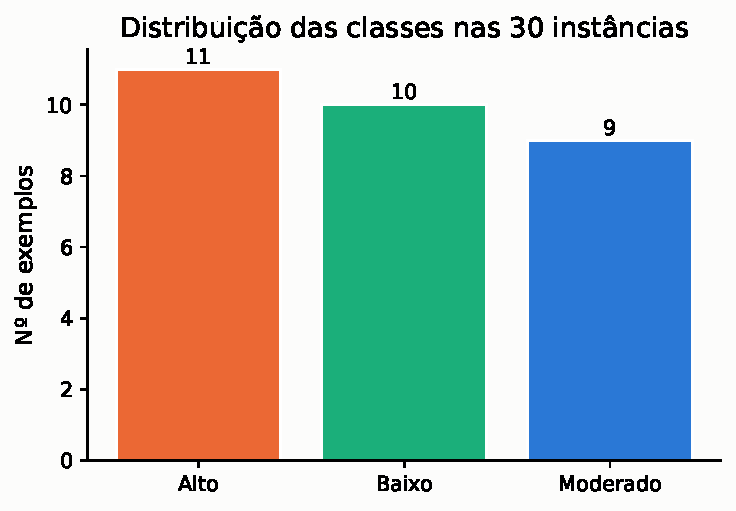
\includegraphics[width=0.72\textwidth]{figures/q02_distribuicao_classes.pdf}
  \caption{Distribuição das classes nas 30 instâncias.}
  \label{fig:dist_classes}
\end{figure}

\subsection{Funcionamento do algoritmo KNN}

O KNN é um algoritmo de aprendizado baseado em instâncias, também conhecido como \textit{lazy learner}. Diferentemente de outros classificadores, ele não constrói um modelo explícito durante o treinamento. Em vez disso, mantém os exemplos disponíveis e utiliza a distância entre eles para classificar uma nova instância.

O processo de classificação pode ser dividido em três etapas:

\begin{enumerate}[leftmargin=2em]
  \item \textbf{Cálculo das distâncias.} Para uma instância de teste $\mathbf{q} \in \mathbb{R}^p$, o algoritmo calcula a distância euclidiana em relação a cada exemplo do conjunto de treinamento:
  \begin{equation}
    d(\mathbf{q}, \mathbf{x}_i) = \sqrt{\sum_{j=1}^{p} (q_j - x_{ij})^2}
  \end{equation}
  \item \textbf{Seleção dos $k$ vizinhos mais próximos.} Depois de calcular as distâncias, os exemplos são ordenados do menor para o maior valor. Os $k$ primeiros são selecionados para participar da classificação:
  \begin{equation}
    \mathcal{N}_k(\mathbf{q}) = \operatorname{arg\,min}_{S \subset D,\ |S|=k} \sum_{\mathbf{x}_i \in S} d(\mathbf{q}, \mathbf{x}_i)
  \end{equation}
  \item \textbf{Votação das classes.} Cada vizinho selecionado contribui com sua classe, e a previsão corresponde à categoria que aparece com maior frequência:
  \begin{equation}
    \hat{y} = \operatorname{arg\,max}_{c \in C} \sum_{\mathbf{x}_i \in \mathcal{N}_k(\mathbf{q})} \mathbb{I}(y_i = c)
  \end{equation}
\end{enumerate}

Caso duas ou mais classes tenham a mesma quantidade de votos, é necessário utilizar um critério de desempate. Isso pode ser feito, por exemplo, considerando a distância dos vizinhos ou a distribuição das classes no conjunto de treinamento.

\subsection{Seleção do hiperparâmetro $k$ via Leave-One-Out (LOO-CV)}

Um dos pontos importantes na configuração do KNN é a escolha do valor de $k$, que determina quantos vizinhos serão considerados em cada previsão. Para definir esse parâmetro, utilizamos a validação cruzada \textit{Leave-One-Out} (LOO-CV).

Como a base possui apenas 30 instâncias, esse método permite aproveitar todos os exemplos na avaliação. O procedimento consiste em retirar uma instância da base para utilizá-la como teste e treinar o classificador com as outras 29. Isso é repetido até que cada uma das 30 instâncias tenha sido utilizada uma vez como teste.

Foram avaliados os valores ímpares $k \in \{1, 3, 5, 7, 9\}$. A escolha de valores ímpares ajuda a diminuir a ocorrência de empates na votação, embora não elimine essa possibilidade em classificações com três classes.

\begin{table}[H]
  \centering
  \caption{Desempenho da validação cruzada Leave-One-Out por valor de $k$}
  \label{tab:loocv_k}
  \renewcommand{\arraystretch}{1.2}
  \begin{tabular}{ccc}
    \toprule
    \textbf{Valor de $k$} & \textbf{Acertos ($/30$)} & \textbf{Acurácia LOO-CV (\%)} \\
    \midrule
    $k = 1$ & 18 & $60{,}00\%$ \\
    $k = 3$ & 19 & $63{,}33\%$ \\
    $\mathbf{k = 5}$ & \textbf{21} & $\mathbf{70{,}00\%}$ \\
    $k = 7$ & 19 & $63{,}33\%$ \\
    $k = 9$ & 18 & $60{,}00\%$ \\
    \bottomrule
  \end{tabular}
\end{table}

O melhor resultado foi obtido com $k = 5$, que acertou 21 das 30 classificações, alcançando 70\% de acurácia. Com $k = 1$, a decisão depende de apenas um exemplo, o que pode tornar o resultado mais sensível a casos específicos da base. Por outro lado, valores maiores de $k$ ampliam a quantidade de exemplos considerados na votação. Neste experimento, a partir de $k = 7$, o desempenho voltou a cair, indicando que a inclusão de mais vizinhos não melhorou a separação entre as classes.

\begin{figure}[H]
  \centering
  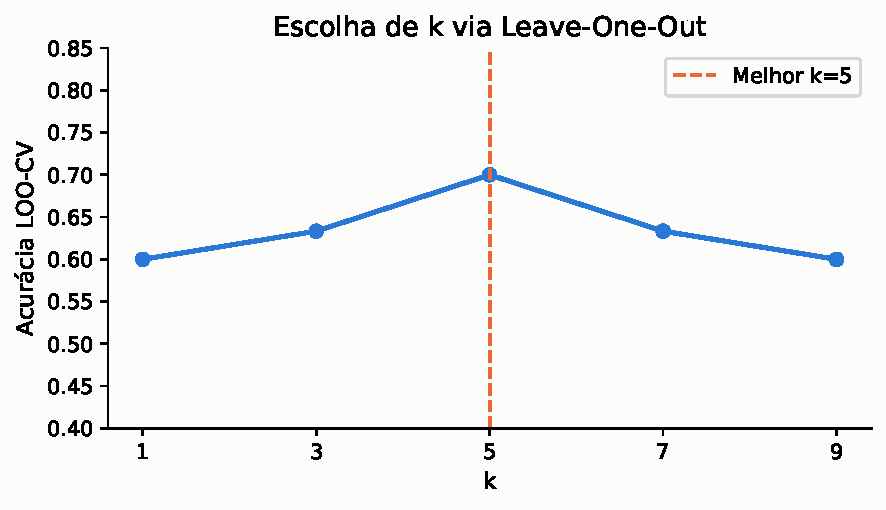
\includegraphics[width=0.68\textwidth]{figures/q02_knn_escolha_k.pdf}
  \caption{Curva de acurácia LOO-CV em função de $k$.}
  \label{fig:loocv_k}
\end{figure}

\subsection{Resultados e análise de desempenho}

Após a escolha de $k = 5$, avaliamos as previsões obtidas pelo procedimento \textit{Leave-One-Out}. As métricas de classificação estão apresentadas na Tabela~\ref{tab:metricas_knn}.

\begin{table}[H]
  \centering
  \caption{Métricas LOO-CV do KNN com $k=5$ sobre as 30 instâncias}
  \label{tab:metricas_knn}
  \renewcommand{\arraystretch}{1.25}
  \begin{tabular}{lcccc}
    \toprule
    \textbf{Classe} & \textbf{Precisão} & \textbf{Revocação} & \textbf{$F_1$-Score} & \textbf{Suporte} \\
    \midrule
    Alto     & 0,71 & 0,91 & 0,80 & 11 \\
    Baixo    & 0,71 & 1,00 & 0,83 & 10 \\
    Moderado & 0,50 & 0,11 & 0,18 & 9 \\
    \midrule
    \textbf{Acurácia global} & \multicolumn{3}{c}{\textbf{70,00\%}} & \textbf{30} \\
    \textbf{Média macro}     & 0,64 & 0,67 & 0,61 & 30 \\
    \textbf{Média ponderada} & 0,65 & 0,70 & 0,63 & 30 \\
    \bottomrule
  \end{tabular}
\end{table}

\begin{figure}[H]
  \centering
  \begin{subfigure}[b]{0.45\textwidth}
    \centering
    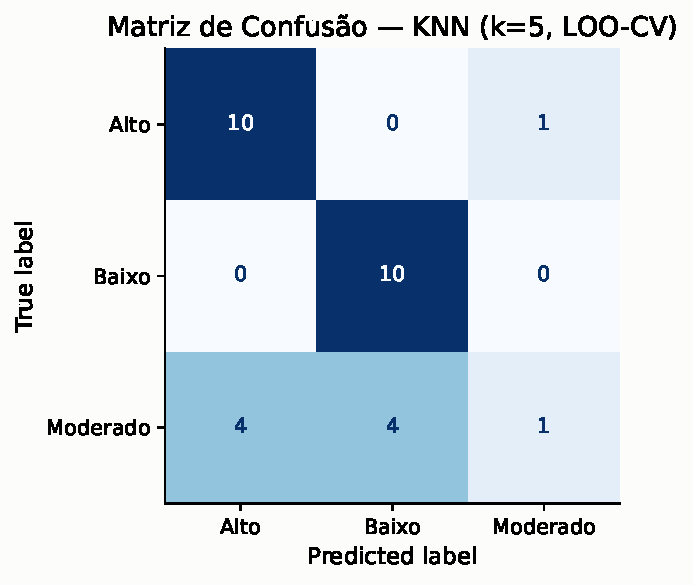
\includegraphics[width=\textwidth]{figures/q02_knn_confusao.pdf}
    \caption{Matriz de confusão ($k=5$)}
    \label{fig:knn_confusao}
  \end{subfigure}
  \hfill
  \begin{subfigure}[b]{0.52\textwidth}
    \centering
    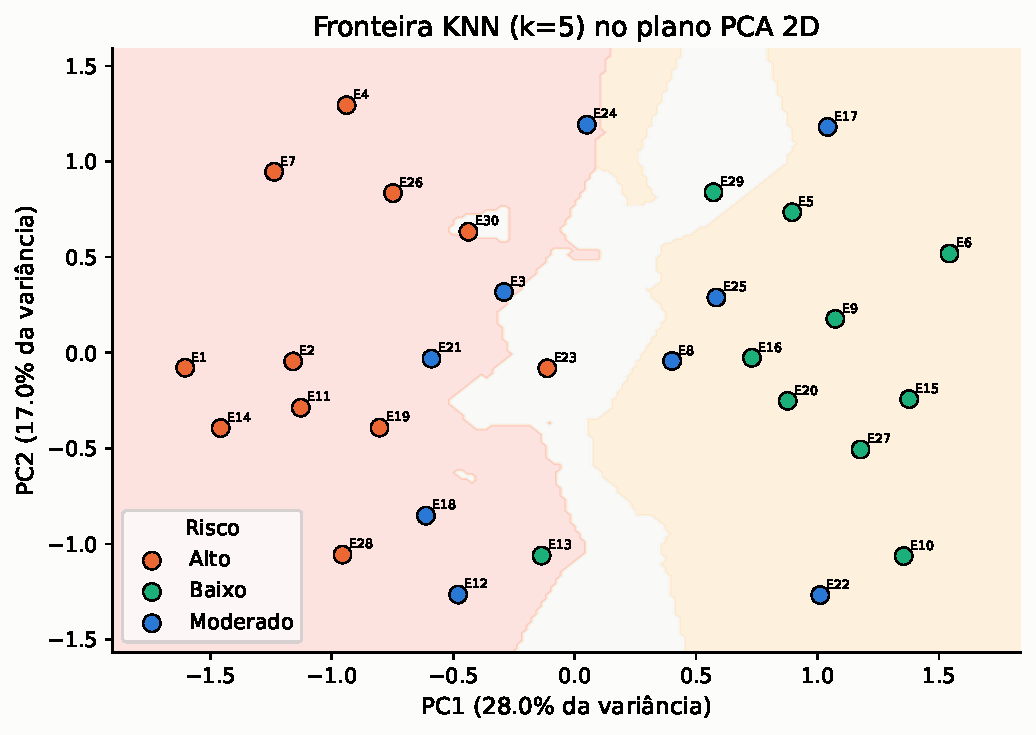
\includegraphics[width=\textwidth]{figures/q02_knn_fronteira.pdf}
    \caption{Fronteira projetada em PCA 2D}
    \label{fig:knn_fronteira}
  \end{subfigure}
  \caption{Visualizações do KNN ($k=5$): matriz de confusão em LOO-CV e fronteira no plano das duas primeiras componentes principais.}
  \label{fig:knn_visualizacoes}
\end{figure}

Os resultados mostram que o classificador teve um desempenho melhor nas classes Alto e Baixo. Foram identificados corretamente 10 dos 11 exemplos de risco Alto e todos os 10 exemplos de risco Baixo.

A maior dificuldade apareceu na classe Moderado: apenas um dos nove exemplos foi classificado corretamente. Os demais foram confundidos com as classes Alto ou Baixo. Esse resultado indica que o KNN teve dificuldade para separar os casos intermediários dos extremos. Como a base é pequena, a posição de poucos exemplos no espaço de atributos pode influenciar bastante a votação dos vizinhos.

Um exemplo que ajuda a entender o funcionamento do algoritmo é a classificação da instância E1, cujo risco verdadeiro é Alto. Seus cinco vizinhos mais próximos são E7, E11, E14, E2 e E4. Todos pertencem à classe Alto. Dessa forma, a votação é unânime e o algoritmo classifica E1 corretamente.

\begin{figure}[H]
  \centering
  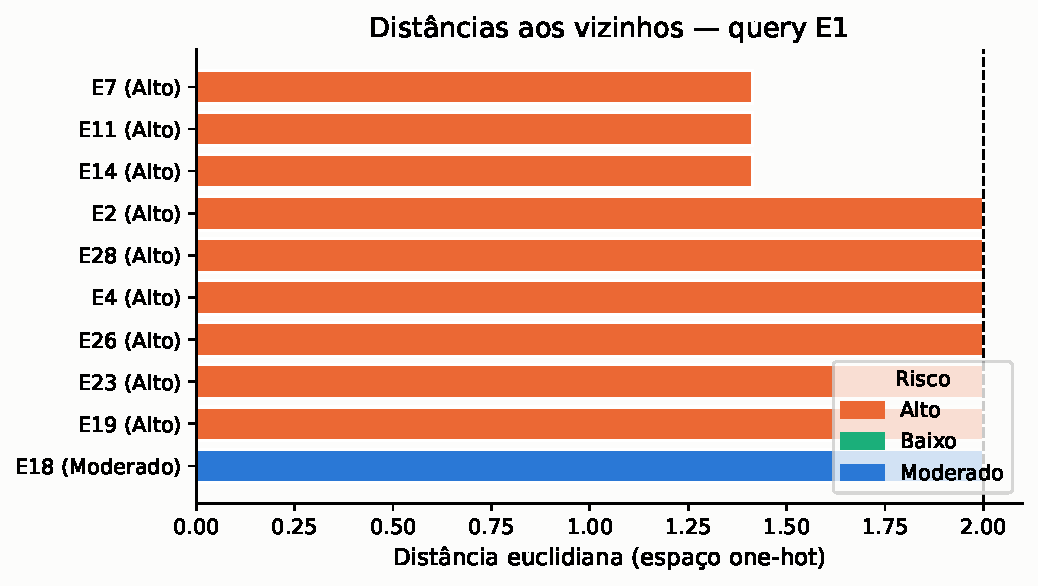
\includegraphics[width=0.72\textwidth]{figures/q02_knn_distancias.pdf}
  \caption{Distâncias aos vizinhos da query E1 ($k=5$).}
  \label{fig:knn_distancias}
\end{figure}

\newpage

% ══════════════════════════════════════════════════════════════════════════════
\section{Questão 3: Chatbot ELIZA, diálogo, algoritmo e evoluções}
\label{sec:q3}
% ══════════════════════════════════════════════════════════════════════════════

\subsection{O chatbot ELIZA e o script DOCTOR}

O ELIZA foi desenvolvido por Joseph Weizenbaum, no MIT Artificial Intelligence Laboratory, entre 1964 e 1966~\cite{weizenbaum1966}. O programa foi criado para simular uma conversa em inglês utilizando regras de reconhecimento e substituição de padrões. A proposta não era fazer com que o computador realmente compreendesse o significado das frases, mas demonstrar como um conjunto relativamente simples de regras poderia levar uma pessoa a acreditar que estava conversando com um sistema inteligente e capaz de demonstrar empatia. Esse comportamento ficou conhecido como efeito ELIZA.

Um dos scripts mais conhecidos do programa é o DOCTOR, que simula uma conversa com um psicoterapeuta da abordagem centrada na pessoa, desenvolvida por Carl Rogers. Nesse tipo de abordagem, o terapeuta costuma ouvir o paciente, fazer perguntas e retomar partes do que foi dito, sem necessariamente apresentar opiniões ou soluções. Isso facilita a simulação, pois o programa não precisa ter um conhecimento aprofundado sobre o assunto discutido: basta identificar determinadas palavras e construir respostas que mantenham a conversa.

\paragraph{Principais funcionalidades.}
\begin{enumerate}[leftmargin=*]
  \item \textbf{Reconhecimento de padrões (\textit{pattern matching}):} o programa analisa a frase e procura palavras-chave e estruturas que correspondam às regras cadastradas, com curingas como \texttt{*}.
  \item \textbf{Montagem das respostas (\textit{reassembly}):} partes da frase original entram na resposta, com substituição de pronomes (\texttt{I}/\texttt{my} $\rightarrow$ \texttt{you}/\texttt{your}).
  \item \textbf{Prioridade das palavras-chave (\textit{keystack}):} cada palavra-chave tem um nível de prioridade; a de maior peso é processada primeiro.
  \item \textbf{Memória de tópicos:} frases com o possessivo \texttt{my} podem ser armazenadas para uso posterior.
  \item \textbf{Respostas alternativas (\textit{fallback}):} quando nenhuma regra produz resposta específica, o programa usa frases genéricas (\emph{``Please go on''}, \emph{``What does that suggest to you?''}).
\end{enumerate}

\subsection{Trecho de diálogo e análise técnica}

O diálogo a seguir é uma adaptação para o português de uma interação clássica apresentada por Weizenbaum (1966), utilizando o script DOCTOR.

{\footnotesize
\begin{verbatim}
[U1] Homens são todos iguais.
[E1] DE QUE MANEIRA?
[U2] Eles estão sempre nos incomodando por causa de alguma coisa.
[E2] VOCÊ CONSEGUE PENSAR EM UM EXEMPLO ESPECÍFICO?
[U3] Bem, meu namorado me fez vir aqui.
[E3] SEU NAMORADO FEZ VOCÊ VIR AQUI?
[U4] Ele disse que eu fico deprimida quase o tempo todo.
[E4] SINTO MUITO EM OUVIR QUE VOCÊ FICA DEPRIMIDA.
[U5] É verdade. Eu sou infeliz.
[E5] VOCÊ ACHA QUE VIR AQUI VAI TE AJUDAR A NÃO SER INFELIZ?
[U6] Eu preciso de um pouco de ajuda, isso é certo.
[E6] O QUE SIGNIFICARIA PARA VOCÊ SE VOCÊ CONSEGUISSE UM POUCO DE AJUDA?
[U7] Talvez eu pudesse aprender a me dar bem com minha mãe.
[E7] FALE-ME MAIS SOBRE A SUA FAMÍLIA.
[U8] Você não gosta de mim.
[E8] O QUE FAZ VOCÊ PENSAR QUE EU NÃO GOSTO DE VOCÊ?
[U9] Você não é uma pessoa de verdade, você é um computador.
[E9] IMPORTA SE EU SOU UM COMPUTADOR?
\end{verbatim}
}

\paragraph{Analisando algumas respostas.}
Em [U3]$\rightarrow$[E3], a palavra \texttt{my}/\texttt{meu} permite capturar o restante da informação e reutilizá-la na resposta, com troca de pronomes: \emph{``Seu namorado fez você vir aqui?''}. Em [U4]$\rightarrow$[E4], uma palavra de estado emocional dispara um modelo de acolhimento previamente definido. Em [U7]$\rightarrow$[E7], a menção à mãe direciona a conversa para o tópico família. Em [U2]$\rightarrow$[E2], \texttt{always}/\texttt{sempre} pede um exemplo específico.

\paragraph{Limitações observadas.}
O programa não constrói uma representação completa da história do usuário entre turnos. Frases com negação, como ``Eu não acho que estou infeliz'', podem acionar a regra de \emph{infeliz}. Em [U9], ao ser acusado de ser um computador, o ELIZA apenas devolve uma pergunta programada. Em [E5], a pergunta sobre ``vir aqui'' parece dar continuidade à conversa, mas resulta da seleção de um modelo associado a \texttt{unhappy}, sem um plano de diálogo.

\subsection{Regras e algoritmo do ELIZA}

O funcionamento do ELIZA segue uma sequência de etapas: normalização e tokenização; varredura de palavras-chave e montagem da \textit{keystack}; casamento com regras de decomposição; substituição pronominal; remontagem no molde escolhido. Se nenhuma regra da palavra-chave atual casar, o algoritmo tenta a próxima da pilha; se a pilha acabar, usa memória de tópicos ou \textit{fallback}.

Exemplo clássico para \texttt{I REMEMBER}: o padrão \texttt{(* I REMEMBER *)} decompõe \emph{``Well, I remember when we lived in Maceió''} em três partes; o molde \texttt{(DO YOU OFTEN THINK OF (3)?)} produz uma pergunta reflexiva a partir do terceiro componente, após a troca pronominal.

Algumas palavras-chave típicas do DOCTOR e suas prioridades aproximadas: \texttt{always} (1), \texttt{what} (2), \texttt{mother}/\texttt{family} (4), \texttt{remember} (5) e \texttt{my} (alta prioridade, com possível armazenamento de tópico).

\subsection{Resposta do ELIZA a cada sentença do diálogo}

A Tabela~\ref{tab:eliza_turnos} relaciona cada turno do usuário à palavra-chave dominante, à transformação e à saída. Em todos os casos, o ``entendimento'' é ilusório: o sistema identifica palavras-chave, decompõe, troca pronomes e preenche um molde.

\begin{table}[H]
  \centering
  \footnotesize
  \caption{Mapeamento turno a turno do diálogo com o script DOCTOR.}
  \label{tab:eliza_turnos}
  \resizebox{\textwidth}{!}{%
  \begin{tabular}{@{}llp{3.4cm}p{4.8cm}@{}}
    \toprule
    \textbf{Turno} & \textbf{Gatilho} & \textbf{Transformação} & \textbf{Saída} \\
    \midrule
    U1$\rightarrow$E1 & generalização / sem chave forte & pergunta genérica & De que maneira? \\
    U2$\rightarrow$E2 & \texttt{sempre}/\texttt{always} & solicita exemplo & Exemplo específico? \\
    U3$\rightarrow$E3 & \texttt{meu}/\texttt{my} & captura + troca pronominal & Seu namorado fez você vir aqui? \\
    U4$\rightarrow$E4 & estado (\emph{deprimida}) & molde de empatia & Sinto muito\ldots deprimida. \\
    U5$\rightarrow$E5 & \emph{infeliz}/\texttt{unhappy} & molde sobre ajuda & \ldots ajudar a não ser infeliz? \\
    U6$\rightarrow$E6 & \emph{preciso}/\emph{ajuda} & pergunta hipotética & O que significaria\ldots ajuda? \\
    U7$\rightarrow$E7 & \texttt{mãe}$\rightarrow$família & direciona o tópico & Fale-me mais sobre a sua família. \\
    U8$\rightarrow$E8 & acusação ao interlocutor & pergunta reflexiva & O que faz você pensar\ldots? \\
    U9$\rightarrow$E9 & exposição (\emph{computador}) & questiona a afirmação & Importa se eu sou um computador? \\
    \bottomrule
  \end{tabular}%
  }
\end{table}

\subsection{Evoluções: PARRY (1972) e AIML / ALICE (1995--2000)}

\paragraph{PARRY (Kenneth Colby, Stanford, 1972).}
Alguns anos depois do ELIZA, Kenneth Colby desenvolveu o PARRY para simular o comportamento de uma pessoa com esquizofrenia paranoica~\cite{colby1972}. Enquanto o ELIZA trabalha principalmente com padrões de texto, o PARRY utiliza variáveis internas de estado emocional --- medo (\textit{fear}), raiva (\textit{anger}) e desconfiança (\textit{mistrust}) --- que influenciam as respostas. A mesma pergunta pode gerar respostas diferentes conforme esses níveis. Em experimentos com transcrições cegas, psiquiatras tiveram dificuldade para distinguir o programa de pacientes reais. A principal evolução em relação ao ELIZA foi a introdução desse estado interno.

\paragraph{AIML e A.L.I.C.E.\ (Richard Wallace, 1995--2000).}
A AIML (\textit{Artificial Intelligence Markup Language}) organiza regras e respostas em categorias XML~\cite{wallace2009}. O A.L.I.C.E.\ (\textit{Artificial Linguistic Internet Computer Entity}) utiliza essa linguagem e venceu o Prêmio Loebner em mais de uma edição. Recursos importantes incluem normalização recursiva com \texttt{<srai>}, contexto com \texttt{<that>} e \texttt{<topic>}, e o \textit{Graphmaster} (árvore de busca para localizar padrões com eficiência). Em relação ao ELIZA, o ganho principal é a organização modular da base, a escala e o controle explícito de contexto --- ainda sem compreensão semântica profunda.

\begin{table}[H]
  \centering
  \small
  \caption{Comparativo das três gerações de chatbots clássicos.}
  \label{tab:chatbots_evolucao}
  \resizebox{\textwidth}{!}{%
  \begin{tabular}{@{}p{2.4cm}p{3.2cm}p{3.4cm}p{3.6cm}@{}}
    \toprule
    \textbf{Critério} & \textbf{ELIZA (1966)} & \textbf{PARRY (1972)} & \textbf{AIML/ALICE (1995)} \\
    \midrule
    Arquitetura & script com padrões e substituição & regras + estados emocionais & categorias XML (Graphmaster) \\
    Modelo interno & pouco desenvolvido & variáveis emocionais & base hierárquica de regras \\
    Contexto & memória simples de tópicos & histórico influenciado pelo estado & \texttt{<that>}, \texttt{<topic>} \\
    Variações & regras fixas de decomposição & heurísticas do comportamento simulado & normalização com \texttt{<srai>} \\
    Domínio & sessão terapêutica & comportamento paranoico & domínio conversacional mais amplo \\
    \bottomrule
  \end{tabular}%
  }
\end{table}

Observando essa evolução, o ELIZA demonstrou como regras simples de reconhecimento de padrões poderiam produzir uma conversa aparentemente natural; o PARRY introduziu variáveis internas; a AIML e o A.L.I.C.E.\ tornaram a construção de chatbots mais organizada. Nenhum desses sistemas possui compreensão semântica semelhante à humana: o que muda é a capacidade de armazenar informações, considerar o contexto, controlar o comportamento das respostas e organizar uma quantidade maior de regras.

% ══════════════════════════════════════════════════════════════════════════════
\newpage
\section{Questão 5: Resumo estendido --- Inferência em LLMs}
\label{sec:q5}
% ══════════════════════════════════════════════════════════════════════════════

Este resumo apresenta os principais conceitos abordados no vídeo \emph{What is LLM Inference? How AI Models Generate Response}~\cite{ibm_llm_inference}, indicado no enunciado da Lista~2. O conteúdo explica o que acontece entre o envio de um \textit{prompt} e a geração de uma resposta por um modelo de linguagem de grande porte (\textit{Large Language Model}, LLM). Ao longo da explicação, são apresentados o papel da inferência, os motores responsáveis por executar os modelos e as etapas que influenciam o tempo de resposta percebido pelo usuário.

\subsection{Treino versus inferência: do modelo treinado à geração de respostas}

O vídeo começa explicando a diferença entre treinar um modelo de linguagem e utilizá-lo depois que o treinamento foi concluído. O treinamento de modelos de grande porte exige uma infraestrutura computacional significativa, pode levar meses e envolver investimentos de centenas de milhões de dólares. Ao final desse processo, o modelo possui um conjunto de parâmetros numéricos, chamados de pesos (\textit{weights}), que armazenam o conhecimento aprendido durante o treinamento.

Esses pesos, por si só, não representam um sistema pronto para conversar ou responder a perguntas. É necessário executar o modelo para que ele processe uma entrada e produza uma saída. Esse processo é chamado de inferência.

Enquanto o treinamento é realizado em etapas específicas do desenvolvimento e da atualização do modelo, a inferência acontece continuamente, sempre que uma aplicação envia uma nova solicitação. É ela que permite o funcionamento de chatbots, assistentes de programação e outras aplicações baseadas em LLMs.

O vídeo também chama atenção para o impacto financeiro dessa etapa. Embora o treinamento tenha um custo inicial muito elevado, a inferência é executada repetidamente a cada solicitação recebida. Quando um modelo passa a ser utilizado por milhões de pessoas, o custo acumulado de execução pode superar o investimento realizado no treinamento. Por isso, reduzir o tempo e o custo de cada inferência é um dos principais desafios para disponibilizar esses modelos em larga escala.

\subsection{O motor de inferência (\textit{inference engine})}

Para que um modelo treinado possa atender às solicitações dos usuários, é necessário um componente de software responsável por coordenar sua execução: o motor de inferência (\textit{inference engine}).

Ele atua como uma camada intermediária entre o modelo e a aplicação que o utiliza. Em vez de simplesmente carregar os pesos e executar cálculos, precisa organizar as requisições recebidas, controlar o uso das GPUs e distribuir o processamento de maneira eficiente.

Entre suas principais responsabilidades estão:
\begin{itemize}[leftmargin=2em]
  \item receber e organizar as requisições enviadas pelas aplicações;
  \item gerenciar a utilização da memória e das GPUs;
  \item definir quais solicitações serão processadas em conjunto;
  \item coordenar a geração e o envio dos \textit{tokens} de resposta.
\end{itemize}

O vídeo apresenta ferramentas como vLLM, Ollama e llama.cpp como exemplos de soluções utilizadas para executar modelos localmente ou em servidores.

Outro aspecto importante é a compatibilidade com APIs. Alguns motores oferecem \textit{endpoints} compatíveis com o formato da API da OpenAI. Isso permite que uma aplicação utilize diferentes modelos ou servidores sem precisar modificar toda a implementação responsável pelo envio das requisições. Assim, a integração entre o modelo e o sistema que o consome fica mais simples.

\subsection{Do texto aos identificadores numéricos: tokenização}

Antes de ser processado pelo modelo, o texto enviado pelo usuário precisa passar por uma etapa chamada tokenização. Nela, a mensagem é dividida em unidades menores, conhecidas como \textit{tokens}.

Um \textit{token} pode representar uma palavra inteira, parte de uma palavra, um número ou até mesmo um sinal de pontuação. Cada unidade é associada a um identificador numérico, chamado de ID. É essa sequência de números que será utilizada pelo modelo durante o processamento, e não o texto original da maneira como aparece para o usuário.

A quantidade de \textit{tokens} gerada depende do texto e do vocabulário utilizado pelo modelo. Por isso, duas mensagens com o mesmo número de caracteres podem resultar em quantidades diferentes de \textit{tokens}.

Essa etapa também tem impacto no custo e no desempenho da inferência. Em muitos serviços, o consumo é contabilizado com base na quantidade de \textit{tokens} de entrada e saída. Além disso, o número de \textit{tokens} do \textit{prompt} influencia o volume de informações que o modelo precisará processar.

O tamanho do vocabulário também merece atenção. Um vocabulário maior pode permitir que determinadas palavras sejam representadas com menos \textit{tokens}, mas aumenta a quantidade de possibilidades que o modelo precisa considerar na etapa de previsão. Portanto, não significa necessariamente que um vocabulário maior resulte em uma inferência mais rápida.

\subsection{Autenticação, roteamento e processamento de múltiplas requisições}

Depois da tokenização, a solicitação segue para a infraestrutura responsável por executar o modelo. Em serviços disponibilizados pela internet, essa etapa pode envolver autenticação por meio de uma chave de API, utilizada para verificar se a aplicação tem autorização para acessar o serviço.

Em seguida, mecanismos de roteamento direcionam a requisição para os recursos computacionais disponíveis. Essa decisão pode considerar fatores como o tamanho da entrada, o modelo solicitado e a capacidade dos servidores naquele momento.

Um ponto importante apresentado no vídeo é que os servidores normalmente precisam atender várias requisições ao mesmo tempo. Processar cada solicitação isoladamente poderia deixar parte da capacidade das GPUs sem utilização. Para explicar esse problema, o vídeo utiliza a comparação com uma padaria que ligasse um forno industrial para assar apenas um pão por vez.

Uma das soluções para aproveitar melhor esses recursos é o agrupamento de requisições (\textit{batching}). Nesse processo, várias solicitações são reunidas para que o hardware consiga processá-las de maneira mais eficiente.

O vídeo também apresenta o \textit{continuous batching}, ou agrupamento contínuo. Nesse modelo, novas requisições podem ocupar os espaços liberados por aquelas que já terminaram, sem que seja necessário esperar todo o grupo finalizar para iniciar outro processamento.

Um componente chamado \textit{scheduler} coordena essa distribuição, organizando quais requisições serão executadas e em que momento. O objetivo é manter os recursos computacionais ocupados de forma eficiente, sem comprometer excessivamente o tempo de resposta de cada usuário.

\subsection{As duas fases da inferência: \textit{prefill} e \textit{decode}}

A geração de uma resposta por um LLM não acontece de uma única vez. O processo é dividido em duas fases principais: \textit{prefill} e \textit{decode}. Cada uma possui características próprias e exige os recursos computacionais de maneiras diferentes.

\subsubsection{Prefill e o KV cache}
Na fase de \textit{prefill}, o modelo processa os \textit{tokens} que compõem o \textit{prompt} enviado pelo usuário. Durante esse processamento, são calculadas e armazenadas informações intermediárias chamadas de \textit{key-value cache} (KV cache).

O KV cache guarda os valores de \textit{keys} e \textit{values} produzidos pelas camadas de atenção do modelo para os \textit{tokens} já processados. Essas informações são reutilizadas durante a geração da resposta, evitando que o modelo precise recalcular tudo a cada novo \textit{token}.

Isso é especialmente importante em conversas longas. Sem esse mecanismo, o processamento dos \textit{tokens} seguintes exigiria repetir parte significativa dos cálculos relacionados ao contexto anterior, aumentando o custo da geração.

O \textit{prefill} costuma ser uma etapa limitada pela capacidade de processamento (\textit{compute-bound}), pois envolve operações matemáticas que podem ser executadas em paralelo sobre os \textit{tokens} de entrada. Seu desempenho depende, entre outros fatores, da capacidade computacional disponível e do tamanho do \textit{prompt}.

\subsubsection{Decode: geração \textit{token} a \textit{token}}
Depois que o \textit{prefill} termina, começa a fase de \textit{decode}. É nesse momento que o modelo passa a produzir a resposta, gerando um \textit{token} por vez.

Em cada etapa, o modelo utiliza os \textit{tokens} anteriores e as informações armazenadas no KV cache para calcular uma distribuição de probabilidades sobre os possíveis próximos \textit{tokens}. Com base nessa distribuição e na estratégia de geração configurada, um \textit{token} é selecionado e adicionado à sequência. O processo se repete até que a resposta seja concluída.

Como cada novo \textit{token} depende dos anteriores, a geração ocorre de maneira sequencial. O KV cache é atualizado durante esse processo para armazenar as informações necessárias aos próximos passos.

Diferentemente do \textit{prefill}, o \textit{decode} costuma ser limitado pela largura de banda da memória (\textit{memory-bandwidth bound}). Isso acontece porque, a cada passo, é necessário acessar os pesos do modelo e as informações armazenadas em memória. Assim, a velocidade de geração depende bastante da rapidez com que esses dados podem ser disponibilizados para o processamento.

De forma simplificada, as duas fases apresentam gargalos diferentes: o \textit{prefill} exige maior capacidade de cálculo sobre a entrada, enquanto o \textit{decode} depende bastante da velocidade de acesso à memória para gerar os \textit{tokens} seguintes.

\subsection{Latência na prática: TTFT e ITL}

Para avaliar o desempenho de um sistema de inferência, não basta observar apenas quanto tempo ele leva para gerar uma resposta completa. Também é importante entender quanto tempo o usuário espera pelo início da resposta e qual é a velocidade com que os próximos \textit{tokens} são enviados.

\begin{table}[H]
  \centering
  \small
  \caption{Métricas de latência apresentadas no vídeo e sua relação com as fases da inferência.}
  \label{tab:ttft_itl}
  \begin{tabular}{@{}p{2.8cm}p{5.6cm}p{5.2cm}@{}}
    \toprule
    \textbf{Métrica} & \textbf{Significado} & \textbf{Relação com as fases} \\
    \midrule
    TTFT (\textit{Time to First Token}) & Tempo entre o envio da solicitação e o recebimento do primeiro \textit{token} da resposta. & Influenciado principalmente pelo \textit{prefill}, além de roteamento e agendamento. \\
    ITL (\textit{Inter-Token Latency}) & Intervalo de tempo entre o recebimento de \textit{tokens} consecutivos. & Relacionado principalmente à velocidade da fase de \textit{decode}. \\
    \bottomrule
  \end{tabular}
\end{table}

As duas métricas ajudam a entender a experiência do usuário durante uma interação com um LLM. Um sistema pode apresentar um TTFT baixo, fazendo com que a resposta comece rapidamente, mas ainda assim gerar os \textit{tokens} seguintes de forma lenta. Da mesma maneira, pode demorar para iniciar a resposta, mas apresentar uma geração rápida depois que o primeiro \textit{token} é entregue. Por isso, analisar TTFT e ITL separadamente permite identificar melhor em qual etapa está o principal gargalo de desempenho.

\subsection{Síntese do caminho entre o \textit{prompt} e a resposta}

Com base nas etapas apresentadas no vídeo, é possível organizar o funcionamento da inferência na seguinte sequência:

\begin{enumerate}[leftmargin=2em]
  \item O usuário envia uma mensagem para um \textit{endpoint}, que pode utilizar um formato compatível com a API da OpenAI.
  \item O texto é convertido em uma sequência de IDs por meio da tokenização.
  \item A solicitação passa pelos mecanismos de autenticação e roteamento da infraestrutura.
  \item O \textit{scheduler} organiza as requisições e utiliza técnicas de \textit{batching} e \textit{continuous batching} para aproveitar melhor as GPUs.
  \item Na fase de \textit{prefill}, o modelo processa os \textit{tokens} de entrada e constrói o KV cache.
  \item Na fase de \textit{decode}, a resposta é gerada \textit{token} a \textit{token}, utilizando as informações armazenadas no KV cache.
  \item Durante a geração, o desempenho pode ser observado por métricas como TTFT e ITL, que representam o tempo até o primeiro \textit{token} e o intervalo entre os \textit{tokens} seguintes.
\end{enumerate}

\begin{figure}[H]
  \centering
  \resizebox{0.92\textwidth}{!}{%
  \begin{tikzpicture}[
      node distance=0.55cm,
      box/.style={draw, rectangle, rounded corners=3pt, align=center,
                  font=\small\sffamily, minimum width=5.2cm, minimum height=0.85cm,
                  fill=ufalblue!10},
      seta/.style={-stealth, thick, draw=ufalblue}
    ]
    \node[box] (a) {Prompt do usuário};
    \node[box, below=of a] (b) {Tokenização (texto $\rightarrow$ IDs)};
    \node[box, below=of b] (c) {Autenticação e roteamento};
    \node[box, below=of c] (d) {Scheduler + batching contínuo};
    \node[box, below=of d] (e) {Prefill: entrada + KV cache};
    \node[box, below=of e] (f) {Decode: geração token a token};
    \node[box, below=of f] (g) {Resposta ao usuário (TTFT + ITL)};
    \foreach \x/\y in {a/b, b/c, c/d, d/e, e/f, f/g}
      \draw[seta] (\x) -- (\y);
  \end{tikzpicture}%
  }
  \caption{Fluxo entre o \textit{prompt} e a resposta, conforme as etapas apresentadas no vídeo.}
  \label{fig:fluxo_inferencia}
\end{figure}

\subsection{Considerações finais}

O vídeo apresenta a inferência sob uma perspectiva de engenharia de sistemas, concentrando-se no que acontece para que um modelo já treinado consiga responder às solicitações dos usuários em tempo real. Em vez de abordar como um LLM aprende durante o treinamento, a explicação mostra como seus parâmetros são utilizados na prática e quais componentes tornam possível executar o modelo em escala.

Nesse processo, os motores de inferência organizam o uso dos recursos computacionais e o atendimento das requisições. A tokenização transforma o texto em uma representação numérica, enquanto as fases de \textit{prefill} e \textit{decode} realizam o processamento necessário para gerar a resposta. O KV cache evita a repetição de cálculos sobre o contexto anterior, e métricas como TTFT e ITL ajudam a avaliar a velocidade percebida pelo usuário.

Um dos principais pontos que ficam da explicação é que o desempenho de um LLM não depende somente do tamanho ou da qualidade do modelo. A infraestrutura utilizada para executá-lo também tem papel fundamental. Em aplicações reais, é necessário equilibrar velocidade, custo e capacidade de atendimento, especialmente quando muitas pessoas utilizam o serviço simultaneamente.

% ══════════════════════════════════════════════════════════════════════════════
\newpage
\begin{thebibliography}{9}

\bibitem{russel2013}
RUSSELL, Stuart J.; NORVIG, Peter. \textit{Inteligência Artificial: uma abordagem moderna}. 3. ed. Rio de Janeiro: Elsevier / Campus, 2013.

\bibitem{carvalho2011}
CARVALHO, André C. P. L. F. et al. \textit{Inteligência Artificial: Uma Abordagem de Aprendizado de Máquina}. Rio de Janeiro: LTC, 2011.

\bibitem{luger2009}
LUGER, George F. \textit{Artificial Intelligence: Structures and Strategies for Complex Problem Solving}. 6. ed. Boston: Pearson, 2009.

\bibitem{lista1_2026}
TENÓRIO, Antonio Rodrigo L. A.; GOMES, Bruno B. F. \textit{Lista de Exercícios 1: Inteligência Artificial}. Notebook \texttt{Lista\_IA.ipynb}, UFAL, 2026.

\bibitem{weizenbaum1966}
WEIZENBAUM, Joseph. ELIZA: a computer program for the study of natural language communication between man and machine. \textit{Communications of the ACM}, v.~9, n.~1, p.~36--45, 1966.

\bibitem{colby1972}
COLBY, Kenneth M.; WEBER, Sylvia; HILF, Franklin D. Artificial paranoia. \textit{Artificial Intelligence}, v.~2, n.~1, p.~1--25, 1971/1972.

\bibitem{wallace2009}
WALLACE, Richard S. The anatomy of A.L.I.C.E. In: EPSTEIN, R.; ROBERTS, G.; BEBER, G. (eds.). \textit{Parsing the Turing Test}. Dordrecht: Springer, 2009. p.~181--210.

\bibitem{ibm_llm_inference}
IBM Technology. \textit{What is LLM Inference? How AI Models Generate Response}. YouTube, 2025. Disponível em: \url{https://www.youtube.com/watch?v=615-yWyS1n0}. Acesso em: 6 nov.\ 2026.

\end{thebibliography}

\end{document}
